\section{Introduction}
The formation of carbonaceous nanoparticles such as soot and Carbon Black (CB) is a complex and multi-scale process that involves chemical reactions, heat transfer, fluid and particle dynamics and spans over wide length ($\sim$ $10^{-12}$ to 1 m) and time ($\sim$$10^{-15}$ to 1 s) scales. Figure~\ref{fig:sootscales} demonstrates the length and time scales relevant to different stages of soot formation from PAH precursors to incipient, nascent and mature soot in flames. Understanding the effect of process parameters on particle concentration, morphology, and composition is not trivial, but crucial due to health and environmental impacts of soot and functional properties of CB.
%Soot particle are broad-band light absorbers~\cite{d2009combustion}, and are emitted in large scales ($\approx$9.5 megatons of soot) acting as the third strongest contributor to climate change after methane and carbon dioxide~\citep{myhre2014anthropogenic}. Because of their small size (classified as $\mathrm{PM_{2.5}}$), soot particles can deposit on lung tissues and penetrate other organs through the bloodstream~\citep{borm2004inhaled} and cause asthma~\citep{niranjan2017toxicological} and heart disease~\citep{nichols2013systematic}. On the other hand, CB is the largest flame-made nanomaterial by production value and volume ($\sim$15 megatons per year with a worth of \$17B) extensively used as a reinforcing agent in rubber and tire industries~\citep{international2016carbon}, and conductive additive in lithium-ion batteries~\citep{Palomares2010}. 
Soot is a broad-band light absorber~\cite{d2009combustion}, and is emitted in large scales ($\approx$9.5 megatons) acting as the third strongest contributor to climate change after methane and carbon dioxide~\citep{myhre2014anthropogenic}. Its fine particulate nature ($\mathrm{PM_{2.5}}$) also raises health concerns~\citep{borm2004inhaled}. In contrast, CB, the largest flame-made nanomaterial by production volume ($\sim$15 megatons annually), plays a critical role in industrial applications, including rubber reinforcement~\citep{international2016carbon} and lithium-ion battery technologies~\citep{Palomares2010}.


\begin{figure}[H]
	\centering
	\begin{tikzpicture}
		\draw (0, 0) node[inner sep=0] 	{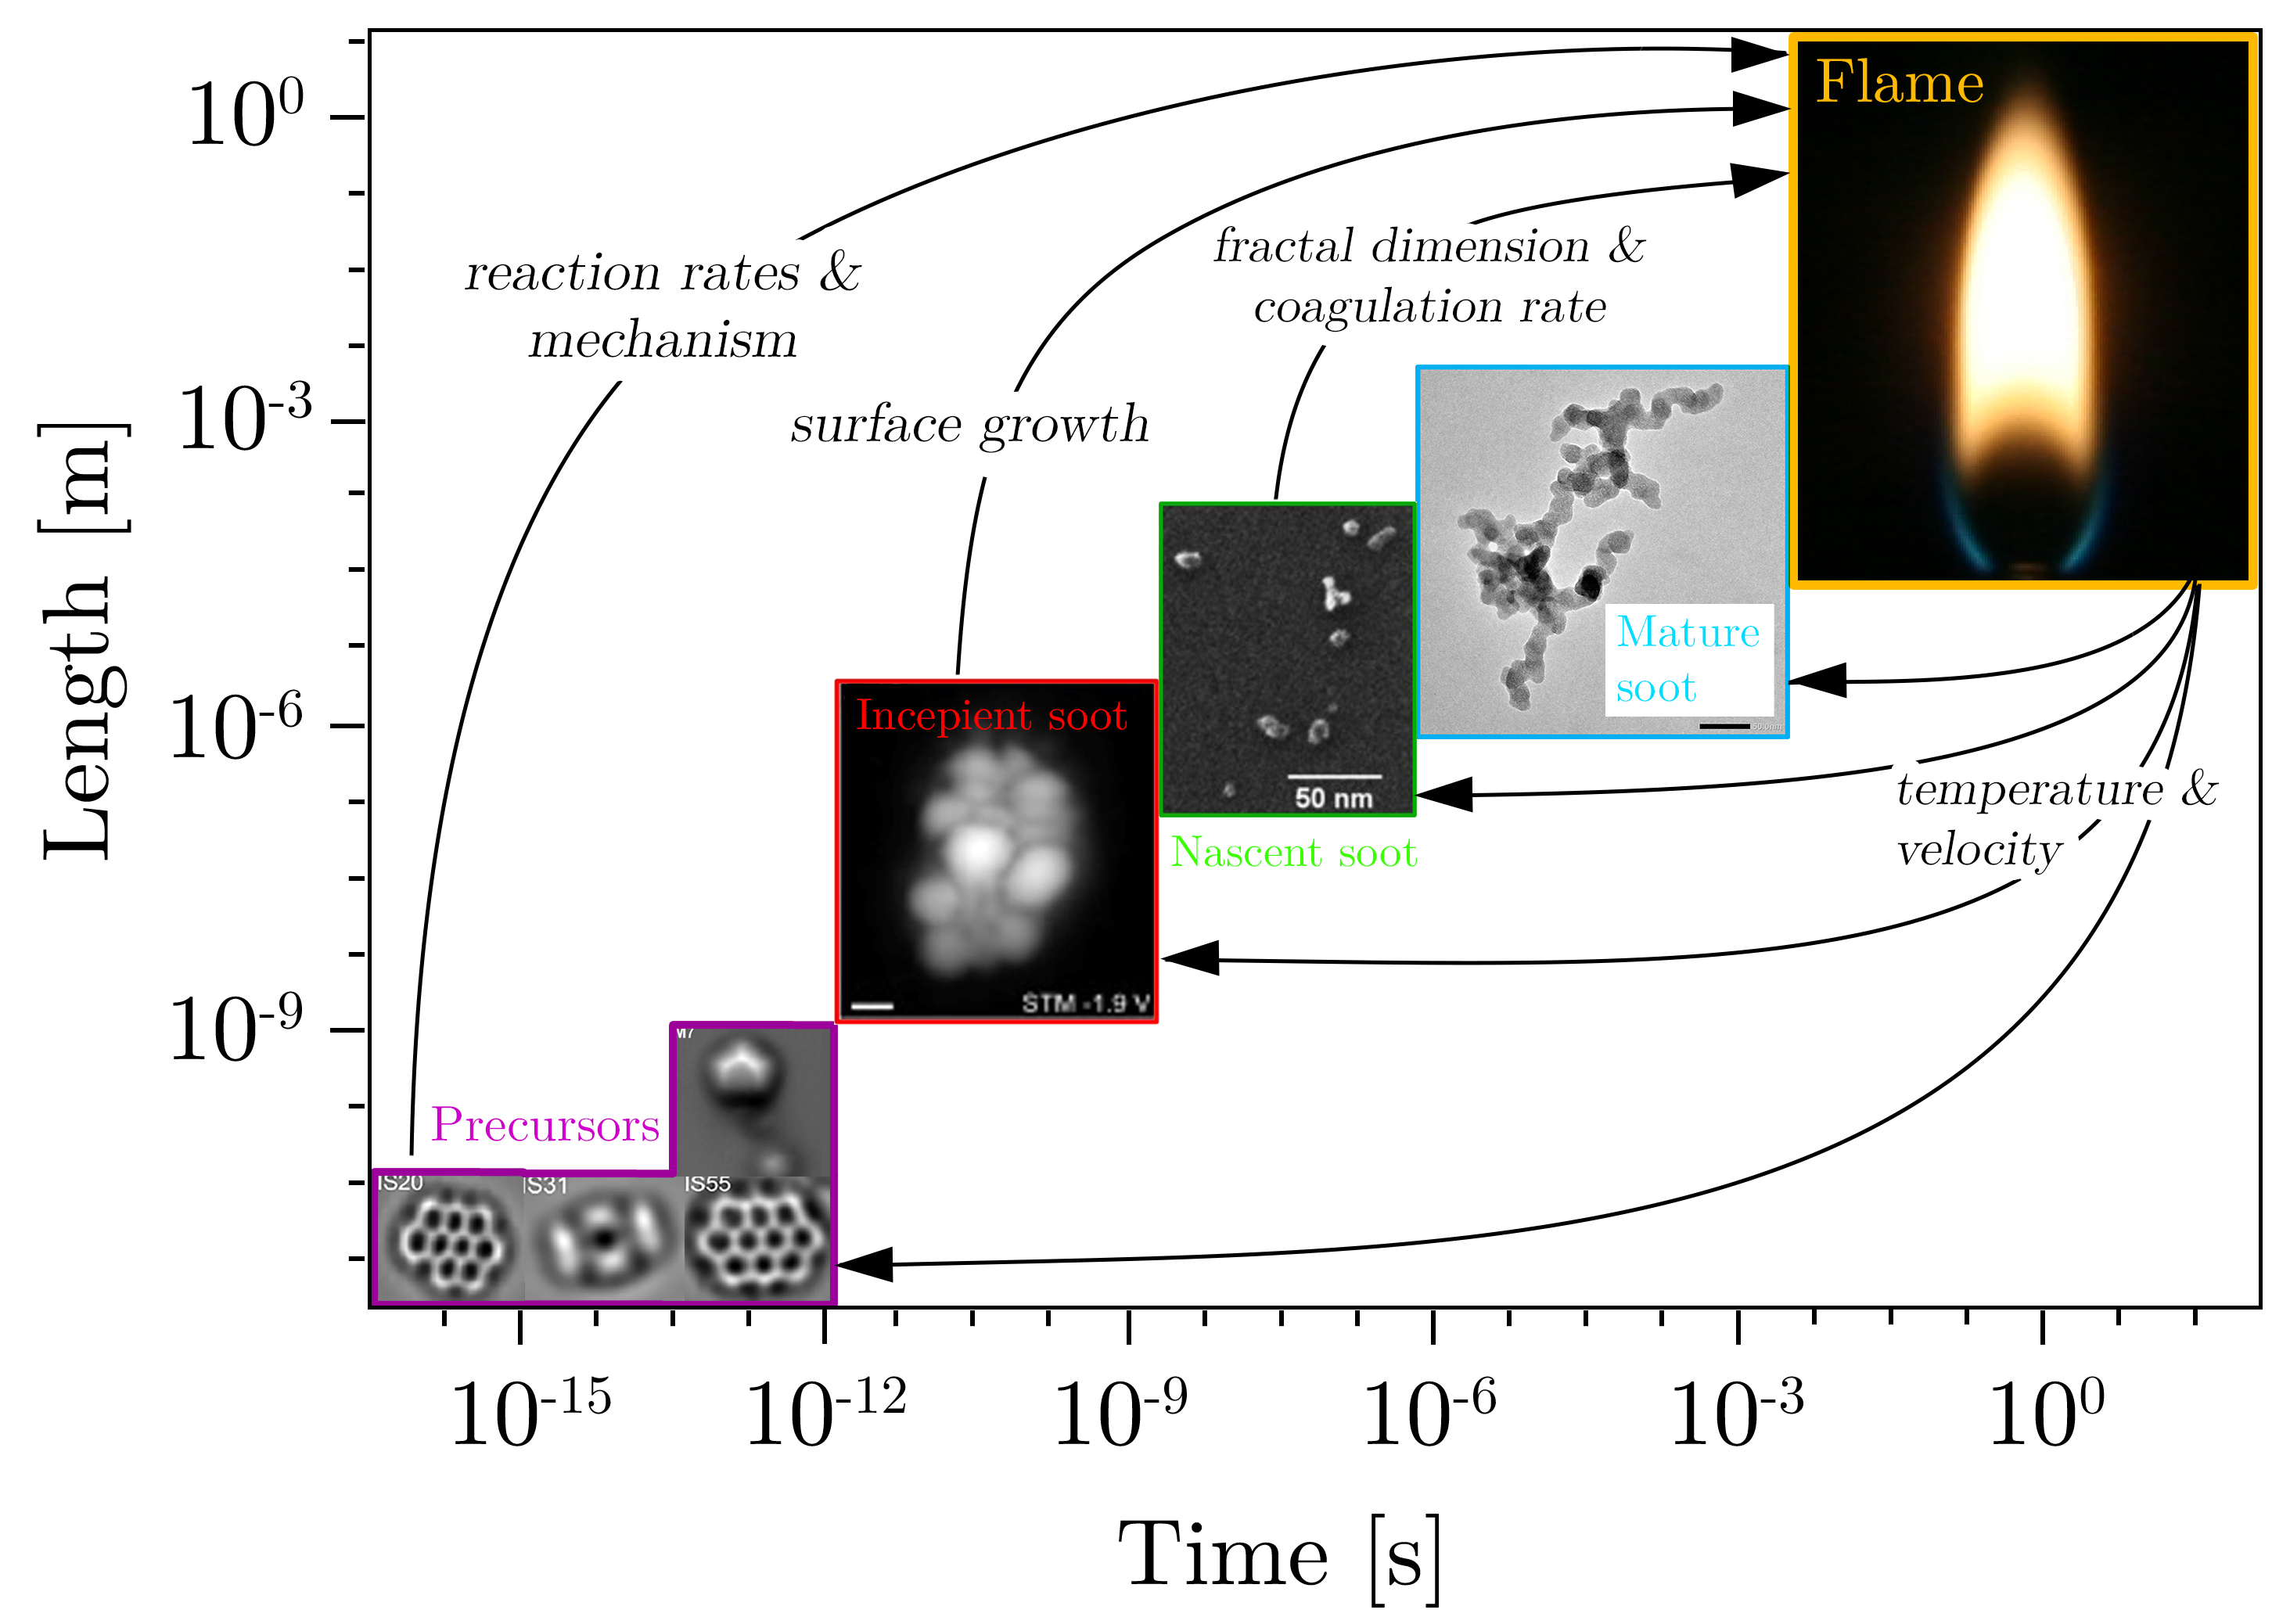
\includegraphics[width=0.8\textwidth]{Figures/Introduction/tlscales.jpg}};
		\draw (-2.7, -1.4) node[text=magenta] {\scriptsize{\cite{commodo2019early}}};
		\draw (-0.1, 0.9) node[text=red] {\scriptsize{\cite{schulz2019insights}}};
		\draw (1.65, -0.23) node[text=green] {\scriptsize{\cite{schenk2013imaging}}};
		\draw (3.15, 0.65) node[text=cyan] {\scriptsize{\cite{kholghy2021morphology}}};					
		
	\end{tikzpicture}
	\caption{The time and length scales of the processes involved in soot formation spans over a wide range including molecular reactions between precursors, surface growth and coagulation of incipient and nascent soot particles and their maturity that depends on the temperature-time-history determined by flame velocity and temperature.}
	\label{fig:sootscales}
\end{figure}

%CB is primarily manufactured by the furnace process which suffers from low mass yield (50-60$\%$ carbon conversion \citep{dames2023plasma}) and excessive emission, generating 4 tons of $\mathrm{CO_2}$ per each ton of product on average~\citep{bansal1993carbon}. Alternative technologies such as plasma-powered reactors for co-generation of hydrogen and CB from methane decomposition has drawn considerable interest~\cite{li2017experimental, fulcheri2023energy, patlolla2023review} thanks to advantages over conventional methods in terms of yield and reduction of $\mathrm{CO_2}$ emission or other pollutants~\citep{cho2004conversion}. 

%Controlling CB yield, structure, morphology and composition is crucial to produce specific grades of CB tailored for various applications in both conventional (e.g. furnace process) and new production methods (e.g. ~\cite{li2017experimental, fulcheri2023energy, patlolla2023review}). However, the effect of process parameters such as feedstock composition, pressure, and temperature-time-history on CB properties has not been completely understood yet due to complexities of gas phase chemistry and CB complicated formation process (as it will discussed in the following). Therefore, there is a clear need for robust computational models to predict yield, particle structure and composition under different process conditions~\citep{park2005influence} and to reduce soot emission in combustion devices.

Controlling CB yield, structure, morphology, and composition is essential for producing specific grades tailored to various applications in both conventional (e.g., furnace process \citep{dames2023plasma}) and emerging production methods~\citep{li2017experimental, fulcheri2023energy, patlolla2023review}. However, the influence of process parameters such as feedstock composition, pressure, and temperature-time history on CB properties remains incompletely understood due to the complexities of gas-phase chemistry and the intricate nature of CB formation (as discussed in the following sections). This highlights the need for robust computational models to predict yield, particle structure, and composition under different process conditions and to mitigate soot emissions in combustion systems.

\textit{"Soot"} and \textit{"Carbon Black"} are distinct materials in terms of chemical properties and synthesis process~\cite{watson2001carbon}. While soot usually refers to the unwanted particulate matter formed during incomplete combustion with variable organic content and a large variation in carbon to hydrogen (C/H) ratio~\citep{watson2001carbon}, CB is commercially produced under highly controlled partial combustion or thermal decomposition of hydrocarbons. However, soot particles generated under controlled laboratory condition has similar structure and composition to CB. The mature soot formed in methane and ethylene premixed flame can reach 95\% elemental C/H ratio~\cite{russo2015dehydrogenation}, which is close to CB composition. The comparison of Transmission Electron Microscopy (TEM) images of industrially produced CB~\citep{singh2018nanostructure} with soot sampled from diesel fuel~\citep{vander2007hrtem, lapuerta2017morphological} indicates similarity of their morphology and structure. Hereafter, soot will be used to collectively refer to carbonaceous nanoparticles produced during combustion/pyrolysis processes.

Soot formation and evolution are believed to begin with the formation of Polycyclic Aromatic Hydrocarbons (PAHs) in the gas phase, followed by the transition of PAHs, which are widely accepted as major contributors to soot inception, into incipient particles—a process known as \textit{soot inception}.
%This description of soot evolution is substantiated by experimental evidence. Transmission Electron Microscopy (TEM) analyses of soot sampled from flames~\citep{lapuerta2017morphological}, reactors~\citep{ono2017experimental}, and engines~\citep{wei2020morphology} across various fuels and process conditions consistently reveal a fractal-like morphology, characterized by agglomerates of primary particles.
The transition of PAHs into incipient soot, or soot inception, remains poorly understood at the level of pathways and elementary reactions~\citep{Wang2011}. This lack of understanding stems primarily from uncertainties in PAH chemistry and the kinetics of PAH growth into soot particles, a process that is highly reversible and thus sensitive to local conditions such as temperature, pressure, and the concentrations of intermediate species~\citep{Wang2011}.

%The growth of PAHs beyond first ring (benzene) is predominantly driven by so-called hydrogen abstraction carbon (acetylene) addition (HACA) mechanism~\citep{frenklach2002reaction} where a hydrogen radical abstracts an hydrogen atom at the edge of PAH, providing a reactive site for acetylene addition. The kinetic reversibility of HACA opens the door for competing pathways such as chain reactions of resonance-stabilized radical (RSR). Propargyl is a prominent example of these radicals, whose combination is known as a major contributor to benzene formation~\citep{fahr1989reactions}. Built on this hypothesis, \citet{johansson2018resonance} proposed a radical-driven growth mechanism by addition of vinyl ($\mathrm{C_2H_3}$) starting from cyclopentadienyl ($\mathrm{C_5H_5}$) to larger hydrocarbon radicals that can survive long enough in high temperatures to react with other radicals, PAHs and unsaturated aliphatic species,
%through radical chain reactions. However, low concentrations of these radicals limit the growth rate through RSR pathways~\citep{frenklach2020mechanism}. Moreover, some of the intermediate steps for radical regeneration such as formation of vinylcyclopentadienyl were shown to be kinetically unfavorable~\citep{frenklach2020mechanism} compared to HACA. Regardless of their mechanistics, these sequential growth mechanisms, termed as \textit{chemical growth} cannot account for rapid soot formation~\citep{frenklach2002reaction} and its nanostructure~\citep{frenklach1988comment}.

%There is abundant but mostly indirect experimental and computational evidence pointing to an alternative collision-based mechanism for soot inception. HRTEM images of nascent and mature soot shows disordered PAH clusters highlighting the role of PAH collisions. 

%The bimodality of particle size distribution (PSD) of nascent soot particles in premixed flames~\citep{zhao2003measurement} indicates that the kinetics of inception is second order in precursor concentration~\citep{abid2009quantitative}. The time-of-flight mass spectrometry (TOFMS) experiments in a 13 kPa acetylene-oxygen flame showed a series of peaks with a periodicity of 500 amu~\citep{happold2009soot}. 

%It is not clear how PAH clusters form and what forces allow the binding to occur and resist dissociation at flames temperatures ($\ge$ 1600 T). \citet{frenklach2002reaction} characterized the clustering as a physical process where the sticking of PAHs upon collision forms dimers held together by Van der Waals (vdW) forces without involving chemical reactions. In fact, \citet{herdman2008intermolecular} found that the binding energy of PAHs dimers due to dispersive and electorstatic forces increases linearly with molecular mass and reaches the limit of exfoliation energy for graphite. However, the entropy barrier of dimerization increases with PAH size making them unfavorable under equilibrium conditions. So, PAHs as large as circumcoronene ($\mathrm{C_{54}H_{18}}$) can only form a dimer to survive flame temperatures~\citep{Wang2011}. However, the concentration of large PAHs are too low to account for the observed number density of soot particles in flames~\citep{totton2012quantitative}. 

%There is also the possibility of PAH clustering governed by non-equilibrium kinetics. PAH molecules can form rovibrationally excited dimer with long enough life-time~\cite{wong2009molecular} to react with H atoms forming covalent bonds. There is another possibility for these clusters to be joined by aliphatic linkages. Micro-FT-IR spectroscopy analysis by \citet{cain2011evidence} showed the ratio of aliphatic-to-aromatic C–H bonds can exceed unity at the flame temperature. Using these findings, they suggested that the aliphatic components in the form of alkyl and alkenyl can covalently bound to aromatic units in soot particles. Although such a mechanism is viable near the flame region, it cannot explain persistent soot inception in the post-flame zone~\citep{zhao2005particle} where the H atom concentration is too low to initiate H abstraction reactions that produce those radicals.

%\begin{figure}[!htbp]
%	\centering
%	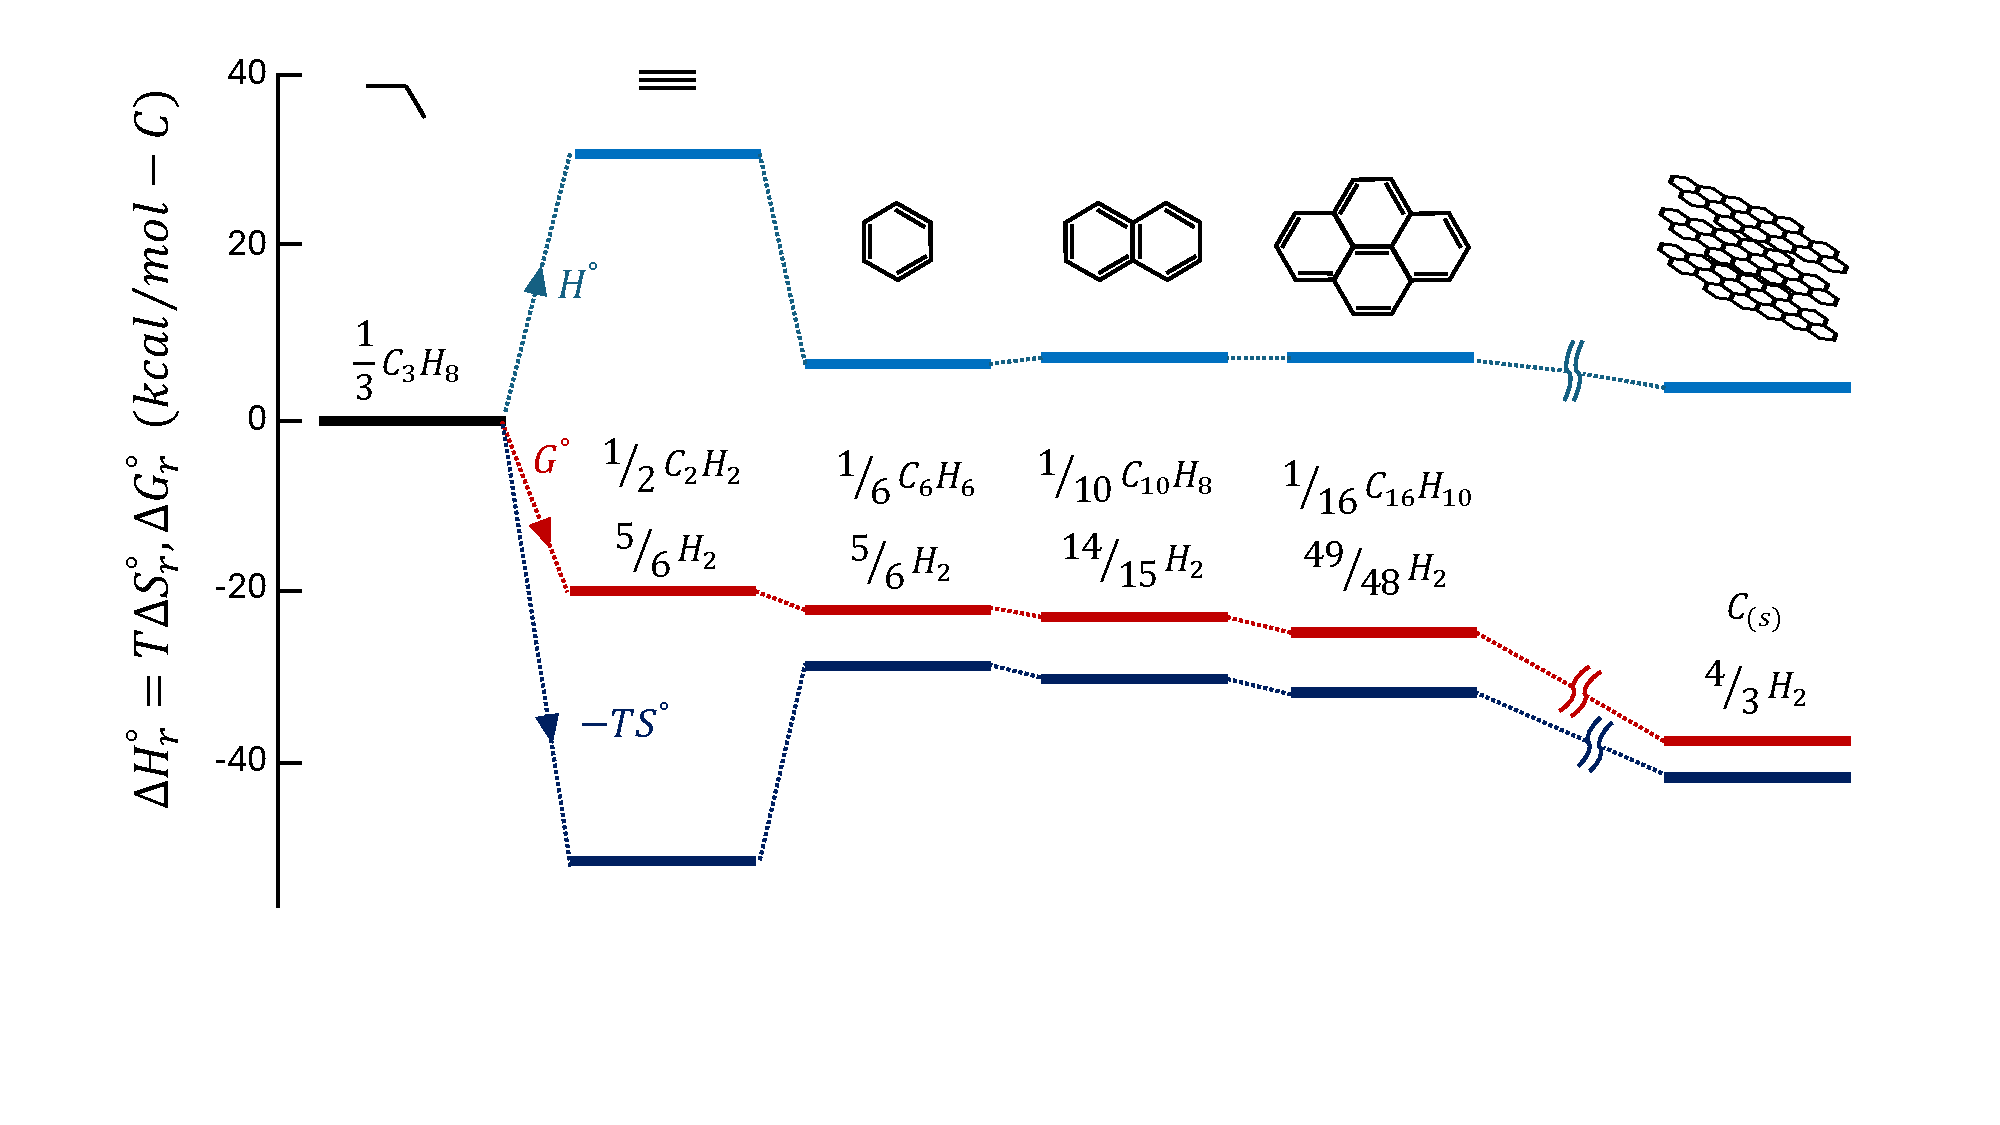
\includegraphics[height=60mm, ]{Figures/Introduction/gibbs_propane.pdf}
%	\caption{Standard enthalpy (${\Delta H}$) and entropy (${T\Delta S}$) contributions to Gibbs function of reaction $\mathrm{\Delta G}$ at 1600 K for carbon formation from propane(reprinted from Ref.~\citep{Wang2011})}
%\end{figure} 

%There are other complicating factors that hinders the fundamental understanding of soot inception such as lack of a decisive criterion to distinguish gaseous molecules from particles~\citep{d2009combustion}, and the overlap of inception with surface growth and agglomeration~\cite{martin2022soot}. Measurement techniques have limited capability in soot detection due to short time and length scales of soot inception and surface growth ranging from pico- to milliseconds and micro- to millimeter~\citep{violi2005relative}. Fig.~\ref{fig:sootscales} demonstrates the length and time scales relevant to different stages of soot formation from PAH precursors to incipient, nascent and mature soot in flames. Moreover, the collected data from measurements might not be true representatives of soot formed at the probed location of the studied process. For example, intrusive diagnostic methods based on thermophoresis or dilution have a sampling probe that can perturb flow dynamics or alter structure and composition of soot~\cite{kholghy2017comparison}. Non-intrusive techniques such as optical methods also rely on assumptions about light absorption and scattering of soot~\citep{shaddix1996laser} and its morphology~\citep{doner2017impact}.


%Despite the gaps in fundamental understanding of soot formation and limitations of diagnostics methods, models have been developed describe the soot inception and growth. These models have been formulated as a set of clear pathways that explain soot inception based on collisions of PAH molecules. They have to be consistent with current knowledge of soot formation mechanisms, feasible to be coupled with chemistry and particle dynamics models, and able to predict soot mass, PSD and morphology observed in flames and reactors.

The classic description of soot inception relies on PAH dimerization where collision of two PAH molecules (monomers in this context) forms a dimer held together by Van der Wales forces~\citep{frenklach1991detailed}. The dimerization is an irreversible process with an efficiency that accounts for the reversibility or dissociation of dimers. The theory postulates that PAH growth continues by sequential addition of monomers forming stacks of dimers, trimers, tetramers and so on to reach a certain mass threshold that marks the emergence of incipient soot~\citep{frenklach1991detailed}, but for practical purposes, a dimer is usually considered as incipient soot. Here, we call this model \textit{Irreversible Dimerization}. 
Irreversible Dimerization has been used to predict soot formation in burner-stabilized premixed~\citep{salenbauch2015modeling, desgroux2017comparative}, counterflow diffusion flames~\citep{wang2015soot, xu2021experimental}, coflow diffusion flames~\citep{kholghy2016core, veshkini2016understanding}. A collision efficiency factor ranging between $10^{-6}$ and 1 is also employed to adjust the inception flux and PAH adsorption rates to achieve desired soot mass and size distribution. PAHs of moderate sizes such as pyrene (4 rings) to coronene (7 rings) have been considered as the starting point of inception due to their thermodynamic instability that justifies the irreversibility at high temperatures~\citep{frenklach1991detailed}. However, the theoretical calculations~\citep{miller1985calculations} and experiments~\citep{sabbah2010exploring} indicated that PAH dimerization is highly reversible in flame conditions. The inception flux of irreversible dimerization is mainly controlled by PAH concentration due to its weak temperature dependence, so it produces new particles at low temperatures (even less than 500 K)~\citep{naseri2022simulating} despite experimental evidence for termination of inception below 1200 K~\citep{sanchez2012polycyclic, cho2016synthesis}. 

%Also, the arbitrary selection of efficiency factors alters the distribution of mass between inception of surface growth that could significantly change soot mass, PSD, and morphology~\citep{saffaripour2014experimental}. 



% Fringe analysis from Jacob's paper 

%  “chemical similarity” hypothesis in "Unified Kinetic Model of Soot Formation in the Pyrolysis and Oxidation of Aliphatic and Aromatic Hydrocarbons in Shock Waves"

% Maybe use discussion in nucleation flame paper to argue for a collision-based proxy inception model 

%  are limited by possible ~\citep{buesser2012design} due to coupling with gas chemistry~\cite{Wang2011}, dependence on local temperature~\citep{gleason2018effect} and pressure~\cite{gleason2021pahs}. It has also been challenging to pinpoint the start of inception because of its short time scales in the order $10^{-9}$ s~\citep{buesser2012design}, the lack of a decisive criterion to distinguish molecules from particles~\citep{d2009combustion}, and the overlap of inception with particle growth and agglomeration~\cite{martin2022soot}. Despite these limitations and challenges, our knowledge about soot formation has significantly increased thanks to advances in diagnostics methods and reaction mechanism development. 





%There is compelling evidence that highlights the role of Polycyclic Aromatic Hydrocarbons (PAH) as the main soot precursors. They are thermodynamically stable enough to withstand dissociation at high flame temperatures~\citep{stein1985high} and observed in stacked layers in High Resolution Transmission Electron Microscope (HRTEM) images of soot primary particles~\citep{Oberlin1984}. 
%\hl{[placeholder for literature review on the role of diradicals and resonantly stabilized radicals in soot inception]}

%But, the two important questions need to be answered: (1) which PAHs contribute most to the inception, and (2) what pathways best describe PAH to incipient soot transition. Purely chemical growth mechanisms are shown to underpredict inception rates and particle size~\citep{frenklach2002reaction}. The bimodality of particle size distribution in premixed flames~\citep{camacho2015mobility} suggests a mechanism second order with respect to the monomer~\citep{Wang2011}. To satisfy these requirements, a collision-based inception was proposed where irreversible polymerization form PAH clusters held together by Van der Wales forces. The theory postulates that PAH growth continues to reach a certain mass threshold that marks emergence of solid particles, but for practical purposes, a dimer is usually considered as incipient soot. 

%In this model, hereafter referred to as \textbf{Irreversible Dimerization}, the collision of two PAH molecules is assumed to form a dimer
% that gains mass via two growth mechanisms: (i) hydrogen-abstraction-carbon-addition (HACA) that assumes soot surface to consist of hydrogenated sites with predefined density that can lose hydrogen and react with acetylene (ii) collision of PAH molecules/clusters with soot particles leading to chemisorption. 





%\citet{eaves2015importance} relaxed the irreversibility assumption, and developed a reversible clustering model to simulate inception using an array of PAHs from naphthalene to benzo-pyrene. Building on that work, 

\citet{kholghy2019role} emphasized on the necessity of chemical bond formation after physical PAH clustering for accurate prediction of volume fraction, primary particle diameter and Particle Size Distribution (PSD) in ethylene coflow diffusion flames. Later, \citet{kholghy2018reactive} proposed the \textit{"Reactive Dimerization"} model which starts with reversible collision of PAHs leading to physical dimers held with vdW forces that are graphitized and form chemically-bonded dimers that serve as soot incipient particles that grow via  coagulation and surface reactions. They also performed a systematic analysis on the contribution of different PAHs, and concluded that one- and two-ring aromatics account for almost all of inception flux in the so-called \textit{"sooting flame"}~\citep{desgroux2017comparative}. However, \citet{frenklach2020mechanism} pointed out that an inception model that initiated with a highly reversible step similar to Reactive Dimerization~\citep{kholghy2018reactive} cannot produce sufficient flux of particles to match measurements of the benchmark burner-stabilized stagnation flame~\citep{abid2009quantitative}. Instead, they proposed the H-abstraction-$\mathrm{C_2H_2}$/Carbon-addition  mechanism~\citep{frenklach1991detailed, appel2000kinetic} (HACA)-driven mechanism where addition of a monomer molecule to its radical activated by hydrogen abstraction forms a stable dimer via an E-Bridge bond formation, and this sequential process continues to form trimers, tetramers, and larger PAH clusters. \citet{blanquart2009joint} proposed a two-step irreversible inception model were self collision of PAH with specified efficiencies results in formation of dimers that collide and subsequently coalesce into an incipient soot.

The gas-phase chemistry of aromatics can be extended to account for chemical growth of incipient soot via surface reactions~\citep{frenklach2002reaction}. This hypothesis, known as “chemical similarity” postulates that the reactions occurring on the soot surface are similar to those involving large molecules of PAHs in the gas phase. It also provides means to describe the rates of surface growth and particle oxidation in
terms of elementary chemical reactions. In other words, it is assumed that the surface of soot particles is made up of lateral faces of larges PAHs covered with C-H bonds.
This is the basis for HACA mechanism~\citep{frenklach1991detailed, appel2000kinetic}  that assumes the soot surface to consist of hydrogenated sites with a predefined density. Mass growth on soot surface requires H-abstraction to form a radical
site, followed by acetylene attack similar to growth of PAH molecules in the gas-phase. The reactivity of these sites changes with time and temperature~\citep{woods1991soot, dasch1985decay}, described as soot aging. For modelling purposes, a temperature-dependent surface reactivity, usually represented by $\alpha$, was introduced to account for the effect of temperature-time-history. \citet{appel2000kinetic} showed $\alpha$ changes with temperature and particle size.

% However, soot mass growth without the presence of H radicals~\citep{singh2006numerical} indicated the incompleteness of the HACA mechanism to describe the entire process of soot surface growth.

Adsorption of PAHs on the surface of soot particles is also a viable growth mechanism~\citep{frenklach1991detailed}, more specifically called physiorption or chemisorption depending on the mechanisms driving the adsorption process~\citep{michelsen2020review}. There is still debate over the stability of adsorbed PAH molecules on soot surface~\citep{obolensky2007interplay}. Following the hypothesis that PAHs are building blocks of soot particles, a mechanism similar to inception is often used to describe  PAH-soot growth.


In typical soot formation processes, such as those occurring in flames and reactors, inception and surface growth are active for only a relatively short duration compared to the total residence time of soot particles. Subsequently, due to high particle concentrations, coagulation becomes the dominant mechanism, rapidly leading to the development of both a Self-Preserving Size Distribution (SPSD)~\citep{lai1972self} and an asymptotic fractal-like structure~\citep{mountain1986simulation, Goudeli2016}.
The collision frequency of agglomerates depends on their evolving fractal-like morphology, with polydisperse agglomerates colliding more frequently than monodisperse ones. This enhancement reaches an asymptotic value of 35$\%$~\citep{Goudeli2016} in the free molecular regime or 82$\%$~\citep{kelesidis2021self} in the transition regime at SPSD, irrespective of primary particle polydispersity.

Particle morphology, governed by inception, surface growth, and agglomeration, can be precisely tracked using mesoscale simulations such as Discrete Element Modeling (DEM)~\citep{Kelesidis2017Flame}. However, these methods are computationally expensive, and integrating them with chemical kinetics in Computational Fluid Dynamics (CFD) frameworks is challenging~\citep{kelesidis2021perspective}. Consequently, their application is often limited to canonical scenarios where particle dynamics are solved independently of chemistry and flow dynamics—For instance, by populating the simulation domain with incipient particles—thereby bypassing the inception step—and neglecting gas removal or addition associated with soot formation~\citep{Kelesidis2017} as it is difficult to have a particle dynamics modeled fully-coupled with gas chemistry. 

As a computationally efficient alternative, particle dynamics can be tracked by Eulerian approaches such as the Method of Moments (MOM)~\citep{kazakov1998dynamic} or Monodisperse Population Balance Models (MPBM)~\citep{kruis1993simple}. Such models only track average particle properties (e.g. moment ratios) and their accuracy could be limited if unrealistic assumptions (e.g. approximating agglomerates as monodisperse and perfect spheres) are used. However, when inception and surface growth are short~\citep{Spicer2002} and high particle number concentrations are formed~\cite{Kelesidis2017}, they lead to rapid attainment of SPSD and agglomerates having asymptotic structure~\citep{Goudeli2016}. In this case a MPBM or MOM can be assembled on a firm scientific basis with accuracy on par with DEM~\citep{Kelesidis2017Flame} and experimental data ~\citep{abid2008evolution, ma2013soot, camacho2015mobility}. Such models can be readily interfaced with CFD simulations~\citep{grohn2012fluid} without significant computational cost, making them ideal for three-dimensional and even turbulent flame simulations. 

The MOM tracks moments of the PSD and estimates average particle properties such as mass~\citep{pratsinis1988simultaneous}, surface area~\citep{blanquart2009joint}, the number of constituent primary particles per agglomerate, ${n_p}$~\citep{kazakov1998dynamic}, or even particle composition~\citep{blanquart2009analyzing} using the ratio of the moments. The MOM with interpolative closure (MOMIC) was developed to predict simultaneous nucleation, surface growth and coagulation of soot agglomerates and estimate its PSD with six equations~\citep{kazakov1998dynamic}. To calculate source terms of the transported moments, additional moments that are not tracked are needed preventing the closure of the system of differential equations with the MOM~\citep{pratsinis1988simultaneous, frenklach1987aerosol}. Thus, often the PSD shape is assumed a priori~\citep{pratsinis1988simultaneous} or extra equations are solved to estimate it~\citep{kruis1993simple}. In contrast, the MPBMs do not have the closure problem and calculate average particle properties by tracking their total concentration, mass \citep{kruis1993simple} and area~\citep{tsantilis2004soft, lindstedt1994simplified}. 

Sectional Population Balance Models (SPBMs), similar to MPBMs but capable of tracking agglomerate and primary PSDs~\citep{Xiong1993}, are widely used in complex laminar~\citep{kholghy2016core} and turbulent flows~\citep{schiener2019transported}. Coupled with relations for fractal-like structure~\citep{matsoukas1991dynamics} and collision frequency~\citep{fuchs1964mechanics}, SPBMs accurately model particle size distribution, morphology, and composition. However, their computational cost rises exponentially with the number of sections~\citep{xiong1993formation} and tracked properties~\citep{kholghy2016core}.
%, so typically only one property (e.g., agglomerate mass) is modeled to reduce expense. In multidimensional simulations, this limitation prevents accounting for fractal-like structure~\citep{smooke2005soot, aubagnac2018soot}, reducing SPBM accuracy in predicting surface growth, coagulation rates, and size distributions. 
SPBMs are gaining attention, due to the recent increase in computational resources, for simulating laminar and turbulent benchmark flames in two-dimensional domains, even with moderately large chemical mechanisms. For example, the CoFlame solver~\citep{eaves2016coflame}, designed to simulate laminar diffusion flames in axisymmetric domains using SPBM, has been employed in numerous studies, demonstrating its ability to accurately capture soot morphological properties~\citep{dworkin2011application, liu2015numerical}. Kholghy et al. extended the SPBM in CoFlame to predict soot maturity by analyzing the equilibrium nanostructure of PAHs within soot primary particles, distinguishing nascent from mature soot based on an isotropic core-graphitic shell structure and surface PAH configuration~\citep{kholghy2016core}. More recent developments have further refined SPBMs by incorporating the persistent radical nature of soot particles, improving the description of nucleation, surface growth, and oxidation in laminar premixed and counterflow flames~\citep{nobili2022modeling}. This approach employs a sectional method in which soot particles are tracked using discrete size bins (BINs), allowing detailed resolution of the size distribution and chemical composition. The algorithm systematically groups PAHs, primary particles, and aggregates into BINs based on carbon atom count and H/C ratio, capturing the evolution of particle size and morphology. By treating large PAHs and soot aggregates as resonantly stabilized radicals, the model reduces the reliance on explicit H-abstraction reactions and improves agreement with experimental data. However, the implementation relies on a customized chemical mechanism, which imposes constraints on modifying individual soot evolution processes, such as inception, growth, or oxidation, without adapting the entire framework~\citep{cuoci2015opensmoke++, cuoci2013computational}.




%\subsection{Soot maturity and its optical properties}
%The maturity level of soot is described as the evolution of physical and chemical properties from incipient to graphite-like mature soot~\citep{michelsen2017probing}. It involves the growth of the graphitic crystallite fine structure of soot within, and perpendicular to, the aromatic layers.~\citep{franklin1951crystallite, haynes1981soot}, known as graphitization, followed by increase in the size ofthe crystallite-layer planes and decrease of the interlayer spacing~\citep{alfe2009structure}. This process is accompanied by the pyrolytic conversion of hydrocarbon species and substituted hydrocarbons toward elemental carbon and increase in the carbon-to-hydrogen (C/H) ratio, known as carbonization. Soot maturity is closely associated with reactivity of surface sites~\citep{camacho2015kinetics}. %At early stages of formation, soot surface is considerably more reactive than that of mature graphitized mature soot. Fig.~\ref{fig:sootmaturity} compares nanostructure of nascent soot composed of disoriented PAH clusters with that of mature soot with a core-shell pattern where disordered core is surrounded by concentrically oriented graphitic layers~\citep{happold2009soot}. The core-shell nanostructure of mature soot strongly depends on process conditions such as pressure, fuel identity, temperature and residence time of the particles. 

%Evolution of soot maturity and morphology impacts its optical properties. Incipient and nascent soot absorb shorter wave lengths ($\lambda<$600 $\mu m$) as opposed to mature soot particles that are broad-band light absorbers~\citep{hurt2000equilibrium}. Non-intrusive optical diagnostic methods such as light extinction (absorption and scattering)~\citep{mcenally1997soot} and Laser Induced Incandescence (LII)~\citep{shaddix1996laser} are widely utilized to measure soot volume fraction, $f_v$ using extinction coefficient and the absorption function, E(m) that depends on soot refractive index, m, soot composition and morphology~\citep{desgroux2013study}.

%\begin{figure}[!htbp]
%	\centering
%	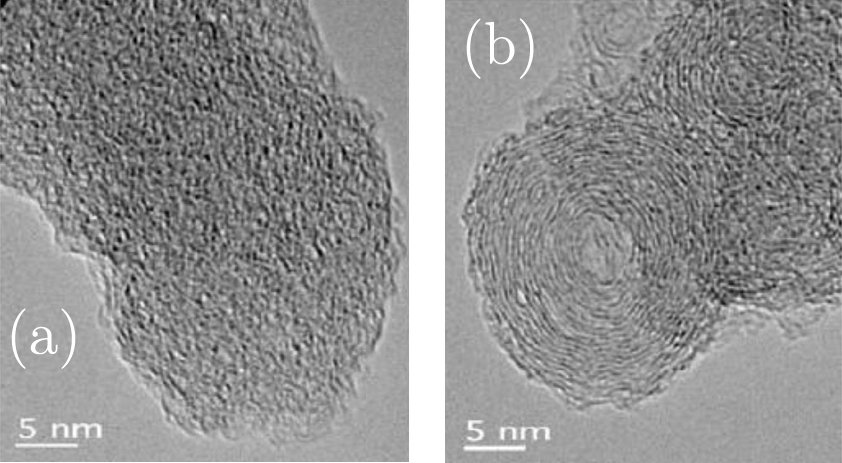
\includegraphics[height=40mm, ]{Figures/Introduction/soot_maturity.jpg}
%	\caption{The HRTEM image of (a) a nascent soot primary particle with disordered internal nanostructure juxtaposed with that of (b) a mature soot primary particle with well-organized cluster near the shell sampled from soot generated by pyrolysis of ethanol at 1250 and 1650, respectively. Reprinted from Ref.\citep{vander2004soot}}
%	\label{fig:sootmaturity}
%\end{figure}


%However, the effects of soot composition, and morphology on its refractive index, and absorption function are not fully understood yet. E(m) of soot at $\lambda=$1064 nm measured by two-color LII measurements increases from 0.193 to 0.349, and 0.226 to 0.340 for ethylene premixed flames with equivalence ratio of $\phi$=2.1 and $\phi$=2.3, respectively when height above burner (HAB) changes from 8 to 14 mm~\citep{olofsson2015evolution}. During acetylene pyrolysis in a shock tube, E(m) of soot particles increases from 0.05 to 0.25 as their primary particle diameter, $d_p$, grows to 20 nm within 1.6 ms~\citep{eremin2011size}. Using m and E(m) of mature spherical soot~\citep{dalzell1969optical} at different HABs neglecting the impact of soot morphology and composition on m~\citep{zerbs2009influence} can overestimate soot volume fraction by 100\%~\citep{kelesidis2021determination}. So, accurate estimation of the evolving optical properties of soot is essential to close the carbon mass balance in the measurements~\citep{kelesidis2021determination}, and analyze reaction kinetics for soot inception~\citep{kholghy2018reactive} surface growth~\citep{appel2000kinetic} and oxidation~\citep{puduppakkam2014soot} that are essential for development and validation of aerosol dynamics models coupled with chemistry to predict soot formation.


%The dependence of soot m on its morphology and composition can be quantified by soot optical band gap, $\mathrm{E_g}$~\citep{bond2006light}. The optical band gap concept was originally proposed by \citet{tauc1966optical} for semi-conductors and later developed for amorphous carbon~\citep{robertson1987electronic}, and it can be used to describe the crystalline character of PAH clusters in soot~\citep{robertson1987electronic}. Incipient flame-made soot with diameters less than 20 nm exhibit quantum dot behavior~\citep{liu2019flame} with 0.7$< \mathrm{E_g}<$2 eV that is larger than $\mathrm{E_g}$ of graphitized soot, 0.12 eV~\citep{liu2019flame}. Optical band gap of organic carbon coated on soot remains nearly constant (~1.8-1.9 eV) over soot evolution~\citep{le2019soot}. In contrast, \citet{russo2020optical} measured soot optical band gap using ex-situ and in-situ methods and showed that $\mathrm{E_g}$ drops from 0.7 eV at HAB= 8 mm to 0.2 eV at HAB=14 mm in an ethylene premixed flame with $\phi$=2.3 as particles grow and become more mature by carbonization. \citet{kelesidis2019soot} correlated the evolving refractive index of soot with its $\mathrm{E_g}$ obtained from quantum confinement theory (QCT)~\citep{liu2019flame} for wavelengths of $\lambda$= 532 and 1064 nm~\citep{kelesidis2019soot} by linear interpolations between that of nascent and mature soot. The proposed relations were then used with soot morphologies obtained from Discrete Element Modeling (DEM) simulations to obtain the evolving Mass Absorption Cross-section (MAC), E(m), and the absorption function ratio of soot (E($\lambda$=532nm)/ E($\lambda$=1024nm)) and compared with measurements~\citep{bejaoui2015measurements, michelsen2010wavelength, cleon2011laser}. Employing the relation in laser diagnostics to reprocess light extinction measurement data resulted in accurate prediction of $f_v$ in moderate ($\phi$=2.34)~\citep{kelesidis2021determination} and rich ($\phi>$3) ethylene premixed flames~\citep{mei2021formation}, and fv along the centerline of a coflow ethylene diffusion flame~\citep{kelesidis2022santoro} which is necessary to close the carbon mass balance in soot generating processes. 

%\subsection{Oxidation}
%Soot oxidation is described as the removal of soot mass by reaction of molecular oxygen ($\mathrm{O_2}$), oxygen radical (O), and hydroxyl radical (OH) from soot surface. Because of its heterogeneous reaction kinetics and mechanisms, oxidation is expected to be sensitive to surface structure and composition. So, oxidation mechanisms depend on soot maturity and temperature-time history. In near stoichiometric and fuel-rich conditions, the contribution of OH radical to soot oxidation is predominant~\citep{neoh1981soot} compared to that of O radicals~\citep{lighty2009soot}. \citet{fenimore1967oxidation} investigated soot oxidation rate for low oxygen
%partial pressures and temperatures from 1530 to 1890 K, highlighted the importance of OH as a major oxidation agent, and attributed the faster rates
%compared to those predicted by \citet{lee1962rate}, to OH oxidation. One approach for describing OH oxidation is by a introducing collision efficiency representing the fraction of collisions of OH with soot particles that resulted in the removal of a carbon atom~\citep{neoh1981soot}. Scanning Mobility Particle Sizer (SMPS) with a two-stage burner also
%showed a collision efficiency of 0.13~\citep{bartok1991fossil}.

%The empirical relation of Nagle and Strickland-Constable (NSC)~\citep{nagle1962oxidation} originally developed for oxidation of pyrolytic graphite have been widely used to describe soot oxidation by $\mathrm{O_2}$. It describes $\mathrm{O_2}$ oxidation rates based on partial pressure of  $\mathrm{O_2}$ and the fraction of reactive edge sites to less reactive basal planes using the graphite analogy for soot. The dominance of edge sites in typical combustion conditions accounts for the relatively small reactivity of soot and basal planes become reactive at high temperature ($>$2500 K)~\citep{lighty2009soot}. $\mathrm{O_2}$ oxidation kinetics was also described with a power-law kinetics \cite{lee1962rate}, and shown to be first order in oxygen concentration~\citep{neeft1997kinetics}. Alternatively, soot oxidation can be explained based on chemical similarity using HACA mechanism assuming that active site are attacked by $\mathrm{O_2}$ and OH leading to loss ot carbon and release of CO.

%A different oxidation regime has been identified for soot at low temperatures (T$<$1000 K) where $\mathrm{O_2}$ diffuses and reacts with bulk soot accounting for most of soot mass consumption~\citep{ma2013soot}.  Internal oxidation compacts the pore network of soot resulting in hollow CB~\citep{kelesidis2022porosity}, diesel~\cite{ishiguro1991microstructural} and biodiesel~\citep{song2006examination} soot particles and increases their SSA up to a factor of four~\cite{ishiguro1991microstructural}. Oxidation can cause fragmentation of soot particles affecting their morphology. The increase in number concentration and the change of soot morphology in lean premixed flames~\citep{xu1997soot} and in the oxidation region of diffusion flames~\citep{puri1993aerosol} was attributed to fragmentation. Such a change in agglomerate morphology has not been observed in fuel-rich conditions, so fragmentation was linked to $\mathrm{O_2}$ oxidation.



%\begin{figure}[!htbp]
%	\centering
%	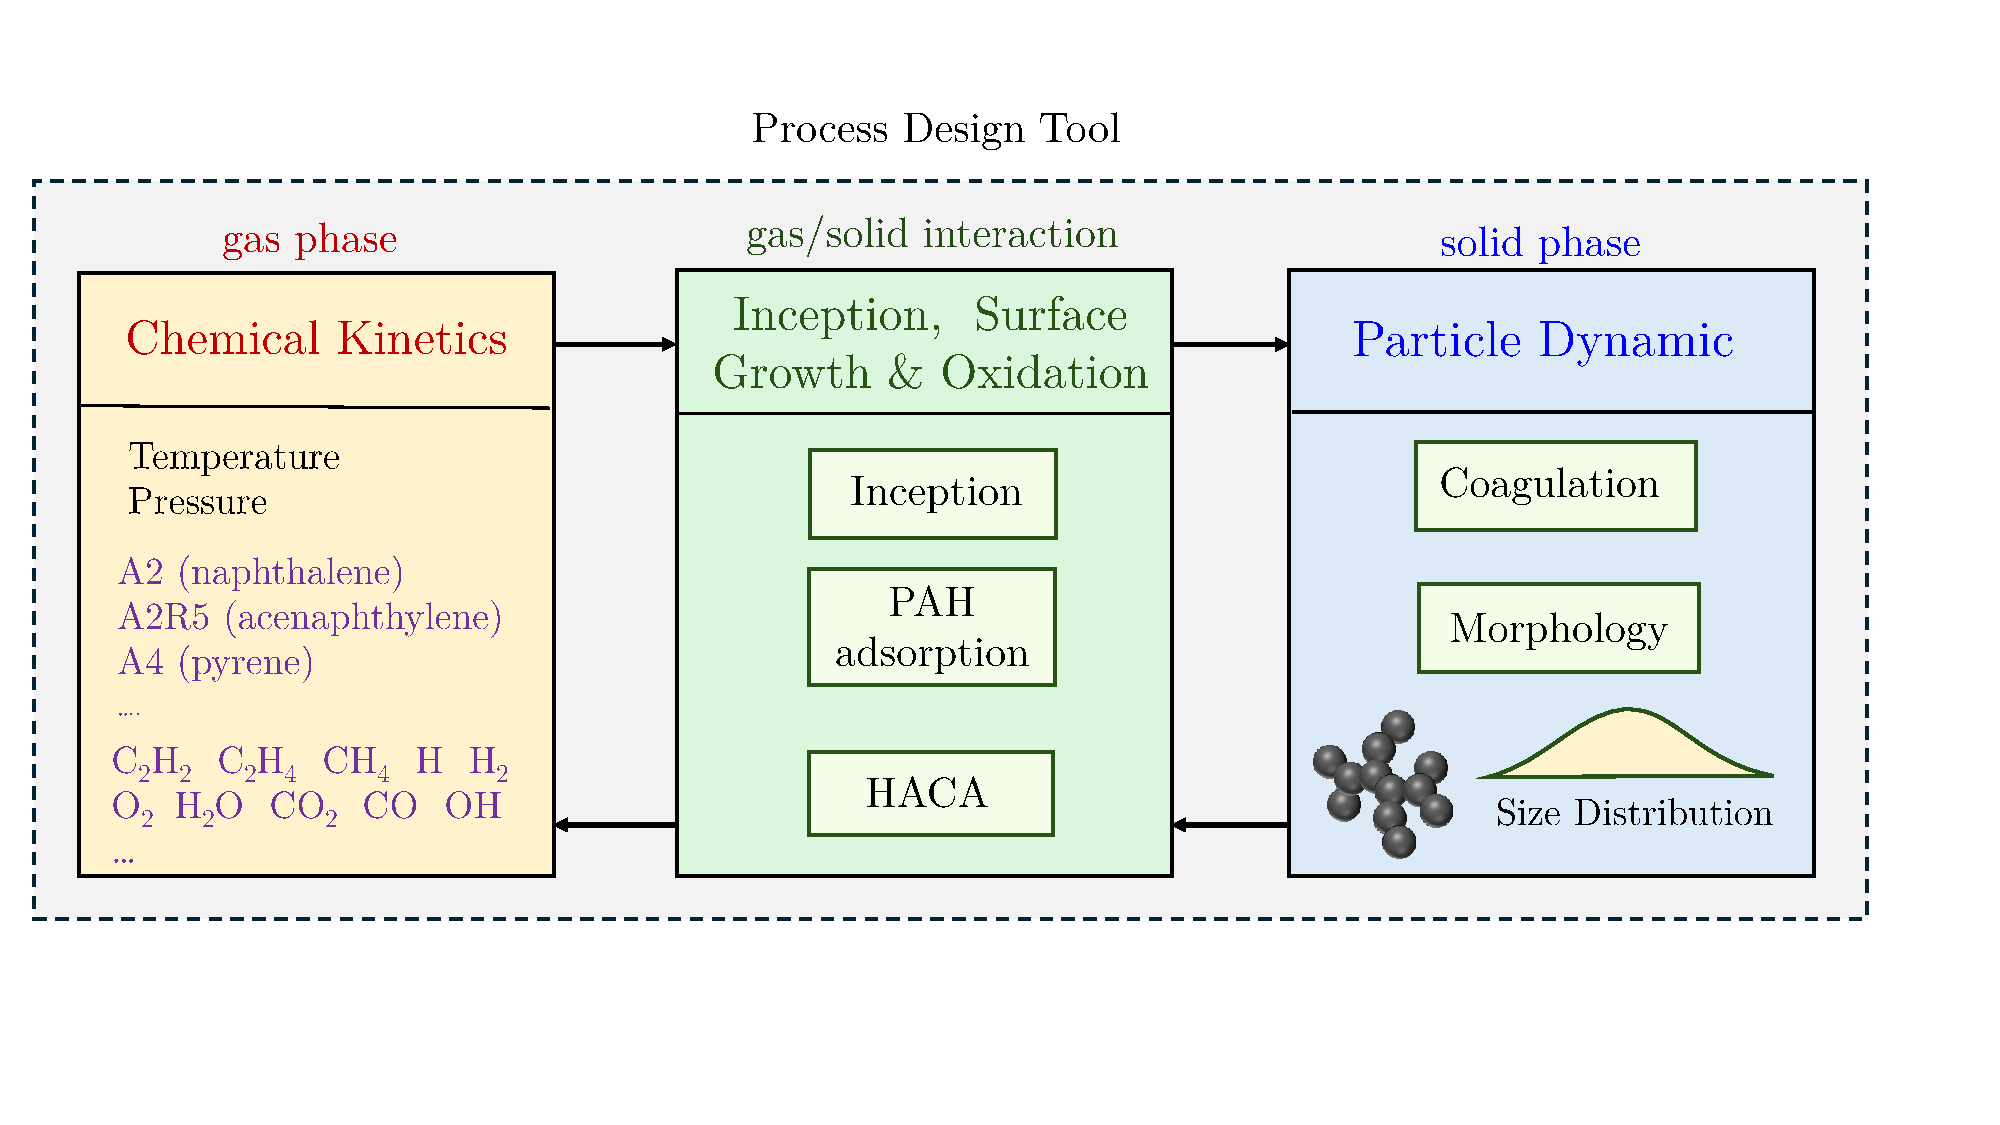
\includegraphics[height=60mm, ]{Figures/Introduction/tooldesign.pdf}
%	\caption{The conceptual structure of developed process design tool that account for gas mixture properties, and soot chemistry involving inception, surface growth and oxidation as well as its coagulation leading to the fractal-like morphology of soot particles}
%	\label{fig:tooldesign}
%\end{figure}

Here, we develop a computational package, called \textit{omnisoot}, which integrates Cantera~\citep{cantera} as a chemistry solver to simulate soot formation in reduced-order dimensions. The package provides a versatile soot model that can be coupled with all reaction mechanisms. Two particle dynamics models—MPBM and SPBM—are incorporated, coupled with various soot inception and surface growth models, offering flexibility to study soot formation alongside gas-phase chemistry. This package facilitates fundamental investigations of soot formation, including pathway analysis, reaction mechanism evaluation, and inception flux estimation, while also supporting process design and optimization of CB production in industrial reactors under diverse fuel compositions, temperatures, pressures, and residence times. The theoretical background and governing equations for sub-models of omnisoot are detailed in subsequent sections, followed by validation against benchmark DEM simulations and verification of mass and energy conservation across all models. Finally, three use cases—shock tubes, flow reactors, and perfectly stirred reactors—demonstrate capability of omnisoot to predict gas chemistry, soot yield, structure, and size distribution.





